\section{Related work}
\label{sec:related}



\subsec{Active Badge}
\label{subsec:badge}


In 1992 the Active Badge system \cite{badge} was presented as an infrared solution capable of provided room-based position tracking. The system has been designed to make use of "active badge" beacons, which can be visualised in figure \ref{fig:badge} in the form of ID cards, a tag eqquiped with an \ac{IR} LED that emitted a unique code for approximately a tenth of a second every 15 seconds.

\begin{figure}[H]
	\centering
		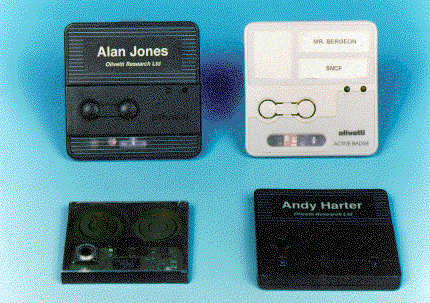
\includegraphics[width=0.5\linewidth]{2.Chapter/badges.gif}
	\caption[Active badge's tags (Ref \cite{badgefig}) ]{Active badge's tags (Ref \cite{badgefig}) }
	\label{fig:badge}
\end{figure}

The decision to utilise \ac{IR} was due to how small and cheap the emitters and detectors are, being capable of operating within a 6 meter range and because \ac{IR} signals aren’t capable of traveling through walls. The signal frequency has two major effects of the system, the first being its impact on the energy consumption of the tags, with such a small frequency allowing for long periods of work on a single battery and the second being its impact on user detection. For the used signal duration and frequency there is a chance of 1/150 for two signals to collide, which leads to a good probability that for a small number of beacons, all will be detected. One downside of such a small frequency signal is that the location of a badge can only be known, at best, to a 15 second granularity.

The position of a user is obtained through the implementation of a network of sensors which act as receivers, listening to badge transmissions, and then forward the obtained information to the master station. The master station is responsible for polling all the sensors on the network, store sighted badges into a database with its associated time, position and ID, data processing and data display. The accuracy of the system is room-based by making use of \ac{CoO} and the properties of \ac{IR}. A beacon in each room would make it so that each beacon is capable of detecting any badges in its room.

One of the issues that surfaced with this system were privacy issues. Due to the system's nature, the position of each badge is known in a centralised station, with the only available option for people who don't wish to be tracked, to disable their tag. Another privacy issue was the security of the system's data with needed improvements to control access to data \cite{badge1}.







\subsec{Active Bat}
\label{subsec:bat}


In 2001 the Active bat system \cite{bat}was introduced, a system capable of tracking various object, each tagged by attaching small wireless transmitters called bats. The system's architecture is composed of small devices named bats, which are to be carried by the objects or people to be tracked, a network of \acf{US} receiver units and several base stations. The receiver network and a deployed bat can be seen on figure \ref{fig:bat};

\begin{figure}[H]
	\centering
		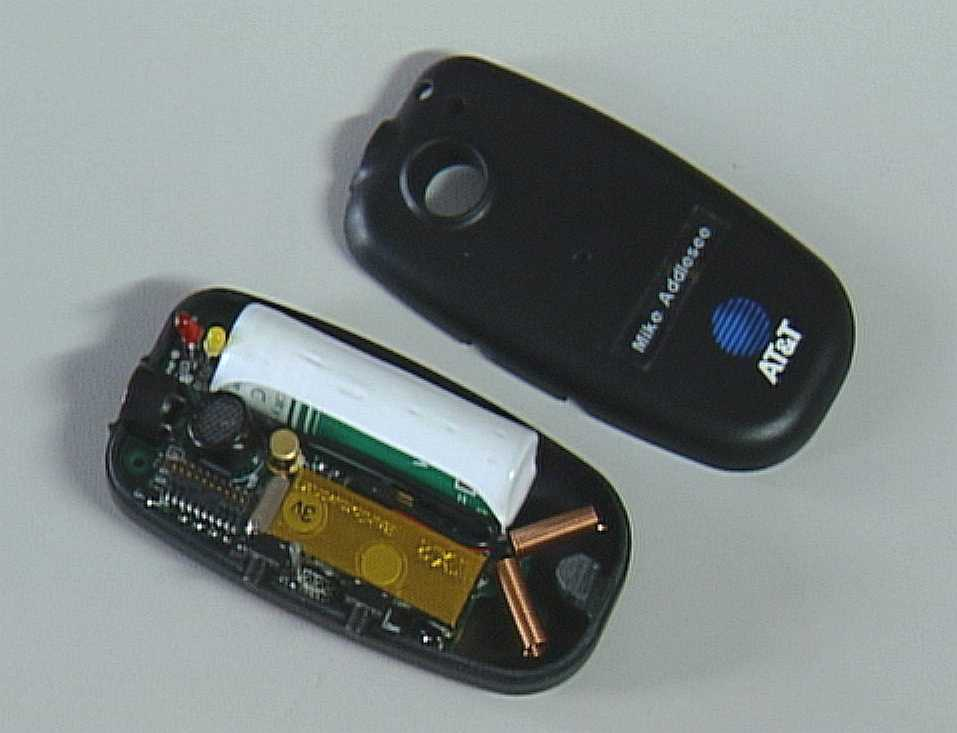
\includegraphics[width=0.5\linewidth]{2.Chapter/batdevice.jpg}
	\caption[Active bat (Ref \cite{batfig}) ]{Active bat (Ref \cite{batfig}) }
	\label{fig:bat}
\end{figure}

 A bat, which can be seen in figure \ref{fig:bat}, consisted of a radio transceiver, controlling logic and a ultrasonic transducer, with each having an associated globally unique ID. A Base station periodically transmits a radio message containing a single unique ID, making it so that the ID's associated bat emits a short pulse of \ac{US}. At the same time, the ultrasound receivers present in the rooms covered by the base station that emitted the radio signal are reset through the wired network. From this point on, the receivers monitor for the expected \ac{US} signal while recording the time spent waiting in order to obtain the signal's \ac{ToA}. With a known speed of sound in air, which can be estimated from the ambient temperature, the \ac{ToA} can be converted into bat-receiver distance.

 The mobile target's position can be obtained through multilateration, in the three dimensional space, if three or more non-collinear receivers' distances are known. This method's accuracy is highly dependent on the distance measurement's accuracy. Distance measurement is affected by signal reflections on objects present in the environment, a problem that was correct by the use of a statistical outlier rejection algorithm. One other issue is the reverberations of the initial signal, which are required to die out before initiating another distance measurement in order to ensure that the incoming \ac{US} signals are from the correct bat. As such the measurement process is divided into time-slots, with each being usable to locate one and only one bat.

 The existent system is capable of being improved in order to also provide the target's orientation. The first option is to place several bats at known points of the rigid object and finding their positions on the 3D space. In cases where multiple bat deployment isn't feasible, if the rigid object is opaque to ultrasound, one single tag might be enough to estimate the objects orientation since any cast signal leaves a shadow on the object \cite{bat1}.

The latest version of the bat included a sensitive motion detector that allowed it to tell the base stations whether it was moving or stationary. Since the base station doesn't require to repeatedly determine the location of a stationary object, the system places these bats into a low-power sleep state which is only removed once the bat stats moving. This implementation allowed for extra power savings while freeing up location-update opportunities for other bats \cite{bat2}.

This system's architecture, much like the Active badge's presented in \ref{subsec:badge}, is tightly controlled and centralised. As such it also incurs into the same privacy issues from the active badge system. Another problem created by this system's technique is the requirement of large numbers of receivers across the ceiling and their placements which require sensitive alignments.


\subsec{Radar}
\label{subsec:radar}

In 2001 the RADAR system was introduced as the first Wi-Fi signal-strength based indoor positioning system \cite{radar}. The system is \ac{RF}-based and its capable of locating and tracking users inside buildings. Radar makes use of signal-strength information obtained through a fingerprint method, presented in subsection \ref{subsubsec:rssi}, to triangulate the user's coordinates. The system's functions in two phases: the data collection phase, where the data is gathered in order to later construct and validate models for signal propagation, which are to be used in the real-time phase to infer user's location. In the offline phase, the type of data collected is the signal strength utilising the methodology already described for the fingerprint method.

Radar's experiments showed \ac{RSSI}'s problems relative to value fluctuation dependent on the user's orientation. This happens due to the existence or not of \ac{LOS} between antenna and base station depending on the orientation, since the user's body may form an obstruction. As such the user's direction was also recorded in the offline phase.

Data processing involve computing the mean, standard deviation and median of \ac{RSSI} for each of the used base stations (three in total) and each combination of x,y and direction. In addition, a building layout information was created which included room and base station's coordinates and the number of walls that obstructed the direct line between the base stations and each of the positions where data was collected. With all this information an accurate signal propagation modal was built.

The basic approach used to obtain a user's location was triangulation, which given a set of \ac{RSSI} measurements at each base station, the user's location is guessed to be the one that best matches the observed data. In addition to this basic strategy, two others approaches were analysed: empirical and signal propagation methods. 

For the first method many variations on the data was studied such as: The number of best matching values used ( K-nearest neighbours (KNN)), with results showing that the benefits of averaging between multiple neighbours isn't very relevant even for small values of k as in this case it doesn't mean that there aren't k physical distinct points. Other factors were studied such as the impact of the number of samples collected or the number of data points and the impact of the user orientation, with the most relevant being the latter, having shown the relevance of collecting data for multiple directions. In general the empirical method was capable of estimating the user's location with high accuracy, obtaining a median error distance between 2 and 3 meters, and with its main drawback being the required effort for building the data set for each physical area of interest. Another issue is the requirement to remake the data collection phase whenever a base stations is moved or there are heavy changes in the environment.

The signal propagation model comes as an alternative to the empirical method for constructing the fingerprint. This method makes use of a propagation model for the signal to generate a set of theoretically-computed signal strength data, similar to the one physically collected. The performance of this method is correlated to the how well the used model is capable of correctly describe the signal. The system's chosen propagation model was Wall Attenuation Factor model (WAF) which takes into consideration obstacles between transmitter and receiver. This model provides a more reasonable way of obtaining data, since it doesn't require detailed and costly measurements. When compared to the empirical method, it was capable of achieving a mean error distance of 4.5 meters, that although it isn't as accurate it can be considerate as a solution when analysing its benefits.


\subsec{Cricket}
\label{subsec:cricket}

The Cricket system \cite{cricket}was developed by the Massachusetts Institute of Technology (MIT) in 2005 and managed to tackle some of the problems existent in the previously mentioned systems. The system makes use of nodes, small hardware platforms, consisting of a RF transceiver, a micro-controller and hardware capable of generating and receiving ultrasonic signals. There are two types of nodes: beacons, which are fixed reference points attached to the ceiling or walls of the building, and receivers, called listeners, which are attached to the objects that need to be tracked. Each beacon periodically transmits a \ac{RF} signal message containing beacon specific information, such as the beacon's unique ID, its coordinates and the physical space associated to the beacon. Whenever a \ac{RF} signal is transmitted, an ultrasonic pulse, which doesn't contain any data, is also emitted thus enabling listeners to measure their distance to the beacons by using the time difference of arrival times of the RF and ultrasonic signals. Each listener utilises the RF signal's beacon information alongside the obtain distances to beacons to compute their space position and orientation. 

When a beacon is deployed it doesn't know its exact position, only a human-readable string which describes its location. In order to compute the recently deployed beacon's position a listener is attached to a roaming device in order to collect distances from the beacons to itself. These distances are used to compute inter-beacon distances, which, when in high enough number, are capable of uniquely define how beacons are located in respect to each other. With this information it is then possible to obtain the beacon's coordinates.

The utilised method for computing distances doesn't require listeners to actively transmit messages which permits cricket to perform well independently to the number of users. This active-beacon passive-listener architecture makes it so that the position of the user isn't tracked by the system thus solving the user privacy that were present in the remaining projects.

\begin{figure}[H]
	\centering
		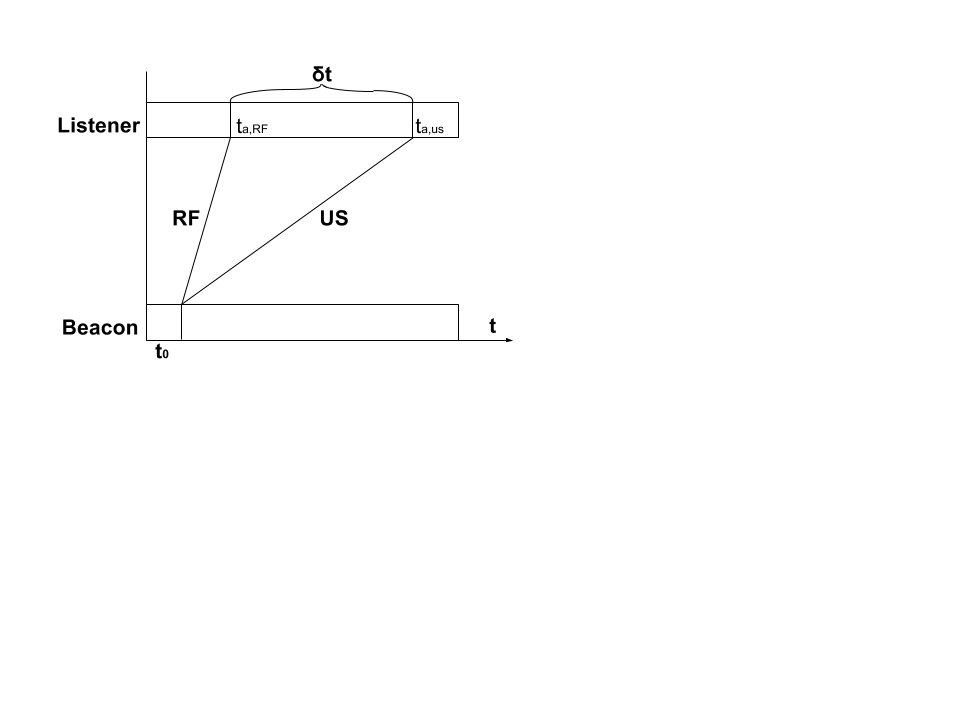
\includegraphics[width=0.5\linewidth]{2.Chapter/cricket-dist.png}
	\caption[Cricket's \ac{TDoA} representation]{Cricket's \ac{TDoA} representation}
	\label{fig:cricket-tdoa}
\end{figure}

Distance measurement is computed through \ac{TDoA} using both \ac{RF} and \ac{US} signals and it can be visualised in figure \ref{fig:cricket-tdoa}. Since the velocity of the \ac{RF} signal is much higher than that of the \ac{US} signal and when considering a direction, the \ac{US} signal lags behind when compared to the other. As such, whenever a listener receives a \ac{RF} signal, it measures the time is takes until the \ac{US} signal arrives, denominated \textit{\delta T}. With knowledge of the speeds of sound and light, the distance between beacon and listener can be obtained from:

$$ \delta t = \frac{d}{v_{US}} - \frac{d}{v_{RF}}  $$

This approach to distance computation is vulnerable to a certain amount of factors such as: Environmental factors since the velocity of sound depends on factors such as temperature, humidity and atmospheric pressure; Lack of \ac{LOS} since in these scenarios there is no \ac{LOS} between the beacon and the listeners, the \ac{US} signal may reach the listener after it has reflected on a surface. Reflection and refraction cause the signal to travel a longer distance than the direct path; Errors in detecting \ac{US} due to the threshold-based approach to detect the signal; \ac{TDoA} associated errors, which are associated to errors from time measurement and errors from detecting the \ac{RF} signal.

In terms of performance, Cricket was capable of a distance measurement accuracy of 4-5 cm within a 80º cone from a given beacon, position accuracy of 10-12 cm and an orientation accuracy of 3º - 5º.



\subsec{BLE systems}
\label{subsec:ble}
	
When looking at what's possible to achieve using the BLE technology there is the example of Apple's creation iBeacon \cite{ibeacon} which was presented in 2013 with the purpose of implementing proximity sensing systems. The device is capable of playing on the broadcaster role and as such its objective is to send nearby compatible receivers certain information. Some examples of application are to track customers or trigger location-based actions on devices such as push notifications or checking in on social media, with practical cases such as the usage of iBeacons by McDonalds to offer special offers to their customers in their fast-food stores. An indoor location system utilising this technology was presented by Jingjing Yang et al \cite{ibeacon1}, where these devices were used to indicate a patient of his whereabouts through the proximity sensing proprieties and this information was later transferred over to a server in order to give clients a variety of different services, from patient counting, to nearby department's information and offer indoor guidance to the nearest available bed. 

When utilising BLE for indoor location the usual metric used to calculate distances is the RSSI. This metric within the context of bluetooth brings to surface several issues such as the fact that RSSI as a metric is very accurate only when the target is within a meter of the beacon, since the value decreases as the inverse of the square of the distance to the beacon . As such when developing solutions for indoor location that require system with high accuracy capable of tracking moving objects, the usage of RSSI can't be utilised without further work. Faragher et al \cite{bleacc} tackled one of the techniques used to improve BLE system's accuracy, fingerprinting, by verifying the effects caused by the device deployment density within the required location. This experiment also puts into evidence one of the downsides of the bluetooth technology being that its scalability is low, besides requiring higher density in order to increase accuracy, due to their low range any need to increase coverage leads to increased costs.


Zonith \cite{zonith} introduced a bluetooth based location system with the objective of tracking the position of workers in dangerous environments. Any device registered in the zonith implemented network would be continuously tracked and accounted for in each of the system's functionalities such as, sounding an alarm whenever a lone worker doesn't move or respond within a time interval (Lone worker protection) or providing a quick an precise location of any worker that has requested for help. This system's installation requires planing of the best locations to place the beacons and number required of beacons in order to be able to provide enough courage and make sure the system provides the required quality.

\subsec{Location description systems}

In order to better understand the existent ways of describing locations it's better to look at existent solutions and the methods that they utilise. The most common method of describing location is through latitude and longitude, much like the \ac{GPS} does, with the biggest example that makes use of it being Google maps. Google maps, through its indoor maps platforms \cite{googlemaps} allows integration of indoor maps onto their google maps. Since google maps uses this type of location description, the indoor component of it follows the same routes. An indoor map on the platform is inserted onto its original geographical location and in the case of having multiple floors, it is possible to navigate through them. This indoor component is of relatively small complexity, likely due to google's reduce investement onto indoor location system, leading to a small amount of indoor specific characteristics. 

Another method is to consider the indoor map as the location reference and utilise a cartesian coordinate system, x and y, to represent a location. Meridian, an indoor location system developed by HP \cite{meridian} which presents functionalities such as route making and push notifications through its beacons, makes use of its platform for insertion of the indoor maps. As such there isn't the outdoor component that google indoor maps has but it allows for utilising a (x,y) system relative to the building map. While no overly complex building description is allowed, it is still possible to indicate the position of specific elements such as restrooms or stores.

Although Meridian already provides some extra level of detail in comparison with google indoor maps, there is another example that should be mentioned called OpenStreetMaps. Although it started much like google, providing global data, due to its openness, many indoor projects surfaced such as OpenLevelUP \cite{openlevel}. This project makes use of OpenStreetMaps' current indoor tagging scheme \cite{opentagging}, which is intented to describe in the most complete and simple way a building. This makes available the number of floors, the type of elemets (room, wall, corridor, etc) and its connectors, like doors and escalators or elevators, allowing to understand clearly the map that is being analysed.
